\documentclass{article}
\usepackage[utf8]{inputenc}
\usepackage{graphicx}
\usepackage{natbib}

\title{\textsf{\textbf{Sistemas Inteligentes - Projeto LaTeX}}}
\author{\textsf{\textbf{Henrique Garcia Leite}}}
\date{\textsf{\textbf{Abril, 2023}}}

\begin{document}

\maketitle

\section{\textsf{Introdução}}

\paragraph{Sistemas inteligentes são ramos que estudam conjuntos de paradigmas que pretendem justificar como um comportamento inteligente pode emergir de implementações artificiais, em computadores. O que pode ser considerado um sistema inteligente é, no entanto, ainda bastante polêmico.}

\paragraph{Considera-se um programa de computador inteligente
quando realiza uma tarefa, que se fosse feita por um ser humano, seria considerada inteligente.
Sistemas complexos não devem ser confundidos com sistemas inteligentes. Um robô que aplica pontos de solda na carroçaria de veículos, apesar de realizar uma seqüência complexa de movimentos, ter requisitos de operação em tempo real e segurança aguçados não é
considerado inteligente.}

\begin{figure}[h!]
    \centering
    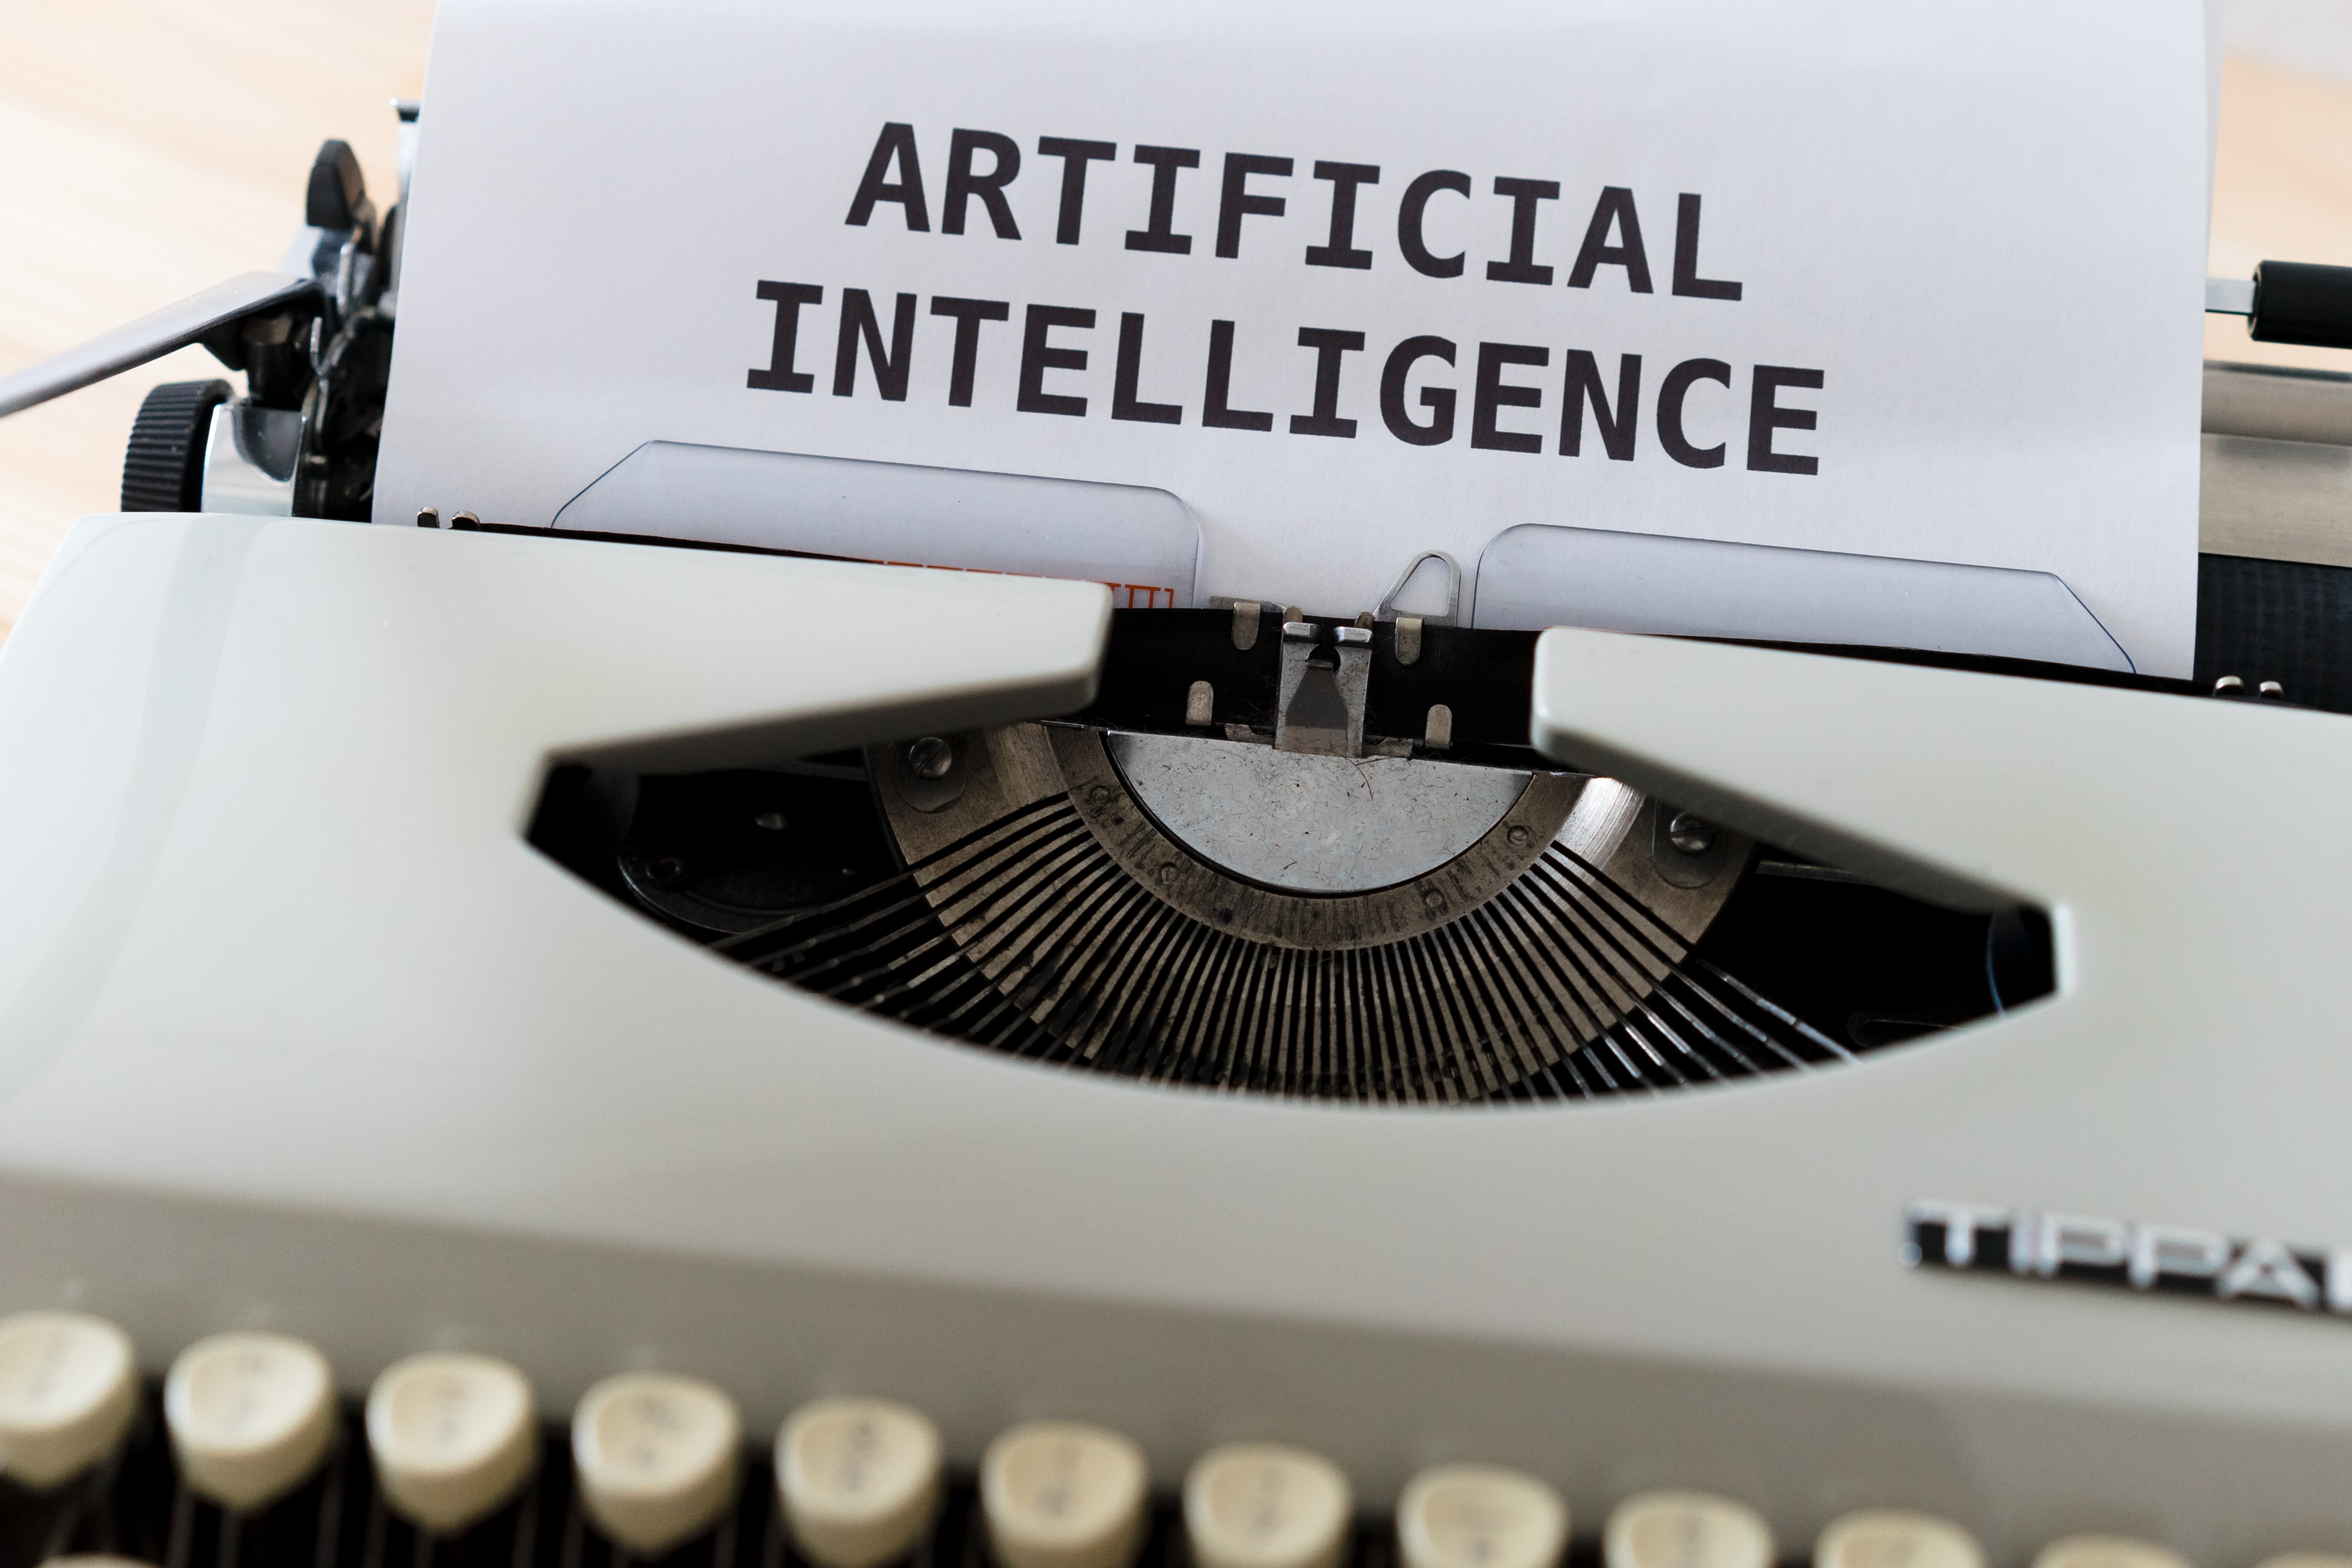
\includegraphics[width=\textwidth, height=6.5cm]{artificial-intelligence.jpg}
    \caption{"Artificial Intelligence"}\cite{IMAGE1}
    \label{fig:my_label}
\end{figure}

\section{\textsf{Relevância}}
\paragraph{Evolução da IA:}
\begin{itemize}
    \item Agindo humanamente (anos 50-70): Teste de Turing \begin{itemize}
        \item Problema: “mito do cérebro eletrônico“
    \end{itemize}
    \item Pensando humanamente (anos 50-60): Simulação cognitiva
    \begin{itemize}
        \item Boas inspirações (GPS, Sistemas Especialistas,...) mas fraca justificativa para os resultados obtidos
    \end{itemize}
    \item Pensando idealmente (anos 60-70): A escola logicista
    \begin{itemize}
        \item Desenvolvimento de formalismos de representação de conhecimento
        \item Problemas: escasez de recursos computacionais, limitação dos tipos de inferências
    \end{itemize}
    \item Agindo idealmente (anos 80 em diante): Agente inteligente
    \begin{itemize}
        \item Abrangente (atividades), unificador (domínios da IA), excelente framework para projeto e análise de programas.
    \end{itemize}
\end{itemize}

\begin{figure}[h!]
    \centering
    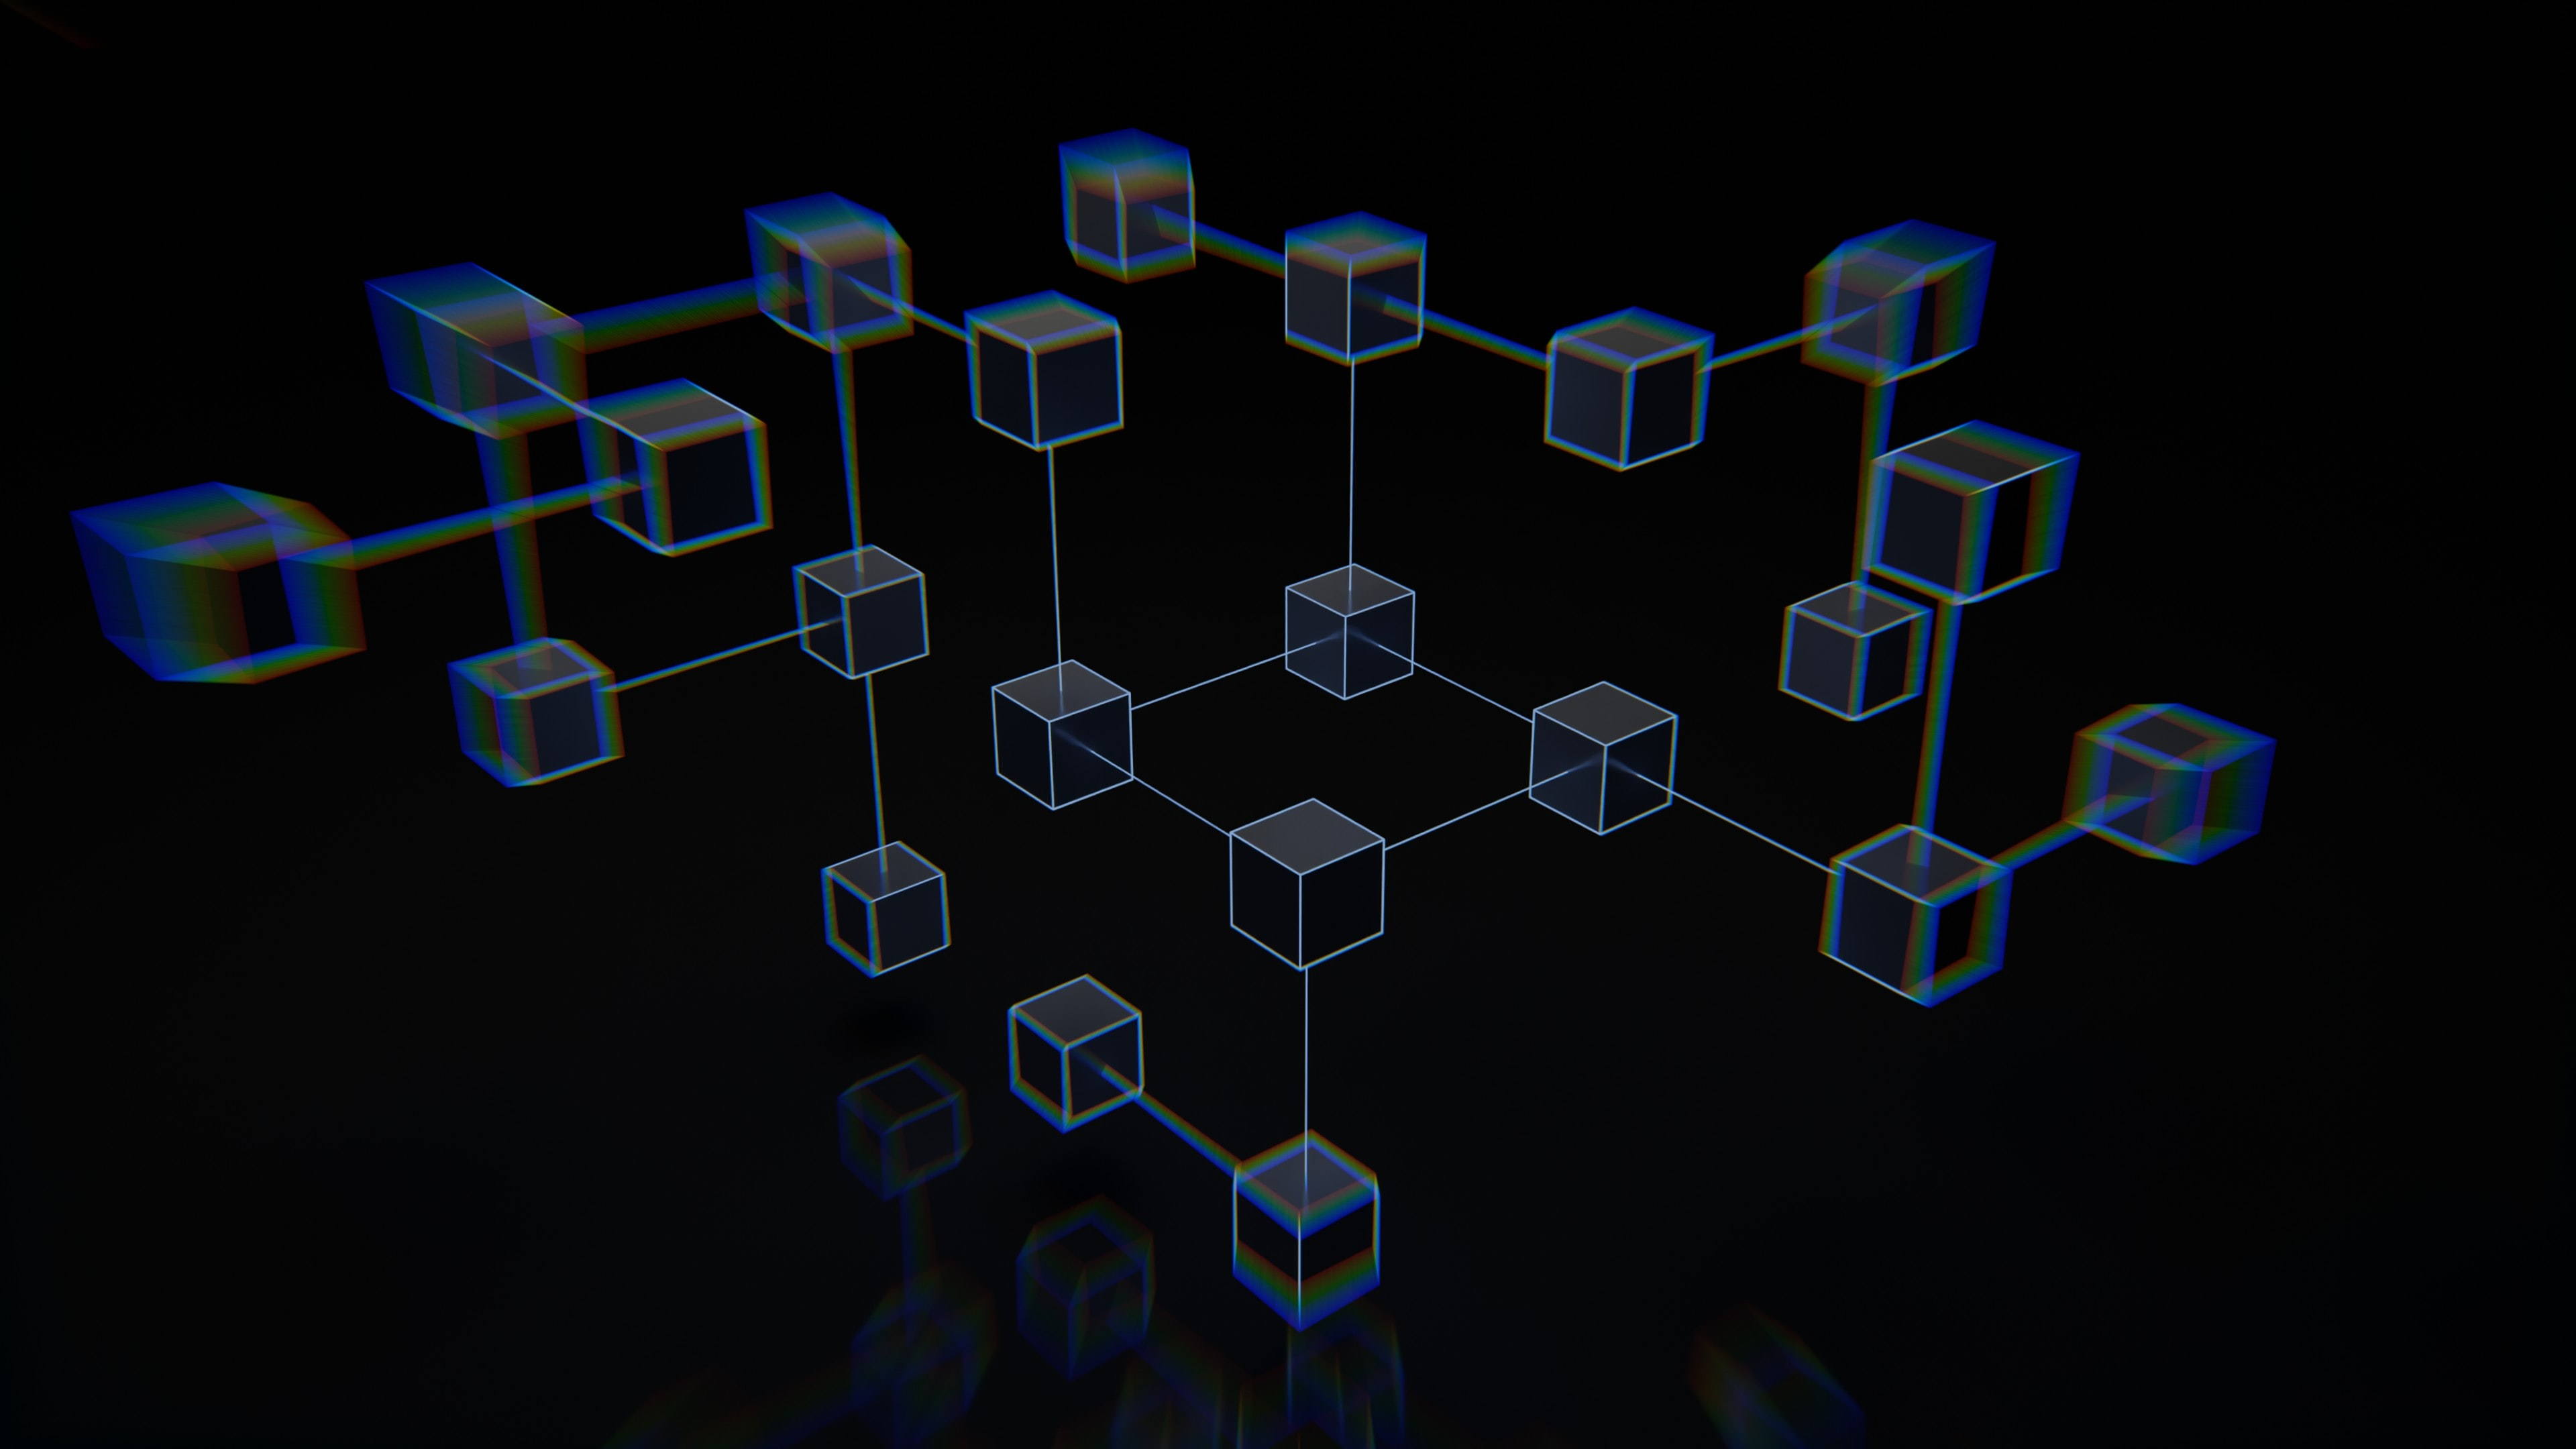
\includegraphics[width=\textwidth]{connected-world.jpg}
    \caption{"Connected World"}\cite{IMAGE2}
    \label{fig:my_label}
\end{figure}

\paragraph{Das aplicações diversas:}
\begin{itemize}
    \item Matemática: demonstração de teoremas, resolução simbólica de equações, geometria, etc.
    
    \item Pesquisa operacional: otimização e busca heurística em geral
    
    \item Jogos: xadrez, damas, go, etc.
    
    \item Processamento de linguagem natural: tradução automática, verificadores ortográficos e sintáticos, interfaces para BDs, etc.
    
    \item Sistemas tutores: modelagem do aluno, escolha de estratégias pedagógicas, etc.
    
    \item Percepção: visão, tato, audição, olfato, paladar...
    
    \item Robótica (software e hardware): manipulação, navegação, monitoramento, etc.
\end{itemize}

\section{Relação com outras disciplinas}

\paragraph{A disciplina de Sistemas Inteligentes tem como pré-requisitos duas outras disciplinas: Algoritimos e estruturas de dados e Lógica para computação}

\paragraph{Também serve como introdução para diversas outras disciplinas: ANALISE IMAG. VISAO COMPUTACIONAL, ANALISE IMAG. VISAO COMPUTACIONAL, OTIMIZACAO, RECUPERAÇÃO DE INFORMAÇÃO etc}

\paragraph{Não apenas para disciplinas voltadas à tecnologia, mas também para disciplinas/cursos fora do escopo, como: Filosofia, Matemática, Sociologia, Linguística, Psicologia, Neuro-Fisiologia, Génetica etc}

\section{Fontes}

\paragraph{CIn UFPE\cite{CinUFPE}}

\paragraph{Sistemas Inteligentes\cite{Sistemas-Inteligentes–if684}}

\paragraph{Artigo Sistemas Inteligentes UNB\cite{Introdução-aos-Sistemas-Inteligentes}}

\bibliographystyle{abbrv}
\bibliography{ref}

\end{document}